\documentclass[a4paper]{article}
\usepackage{Style/DaVinci2019}
\usepackage{enumitem} % http://ctan.org/pkg/enumitem
\usepackage[none]{hyphenat}
\usepackage{hyperref}
\usepackage{pdfpages}

\newcommand{\Abr}{Administrative Regulations} % Bestuursregelement
\newcommand{\Asta}{Bylaws} % Statuten
\newcommand{\Ahr}{House Rules} % Huishoudelijk Regelement
\newcommand{\Asr}{Safety Rules} % Veiligheidsregelement
\newcommand{\Awr}{Contest Rules} % Wedstrijdregelement
\newcommand{\Ajv}{Annual Report} % Jaarverslag
\newcommand{\App}{Privacy Policy}
\newenvironment{g}{\color{grey}}{}

\setTitle{House Rules}
\setSubtitle{April 2019 - {\color{accent2}Proposal for GA 33}}
\enableFooter
\linenumbers
\setFooter{Huishoudelijk Regelement}

\begin{document}
\newpage
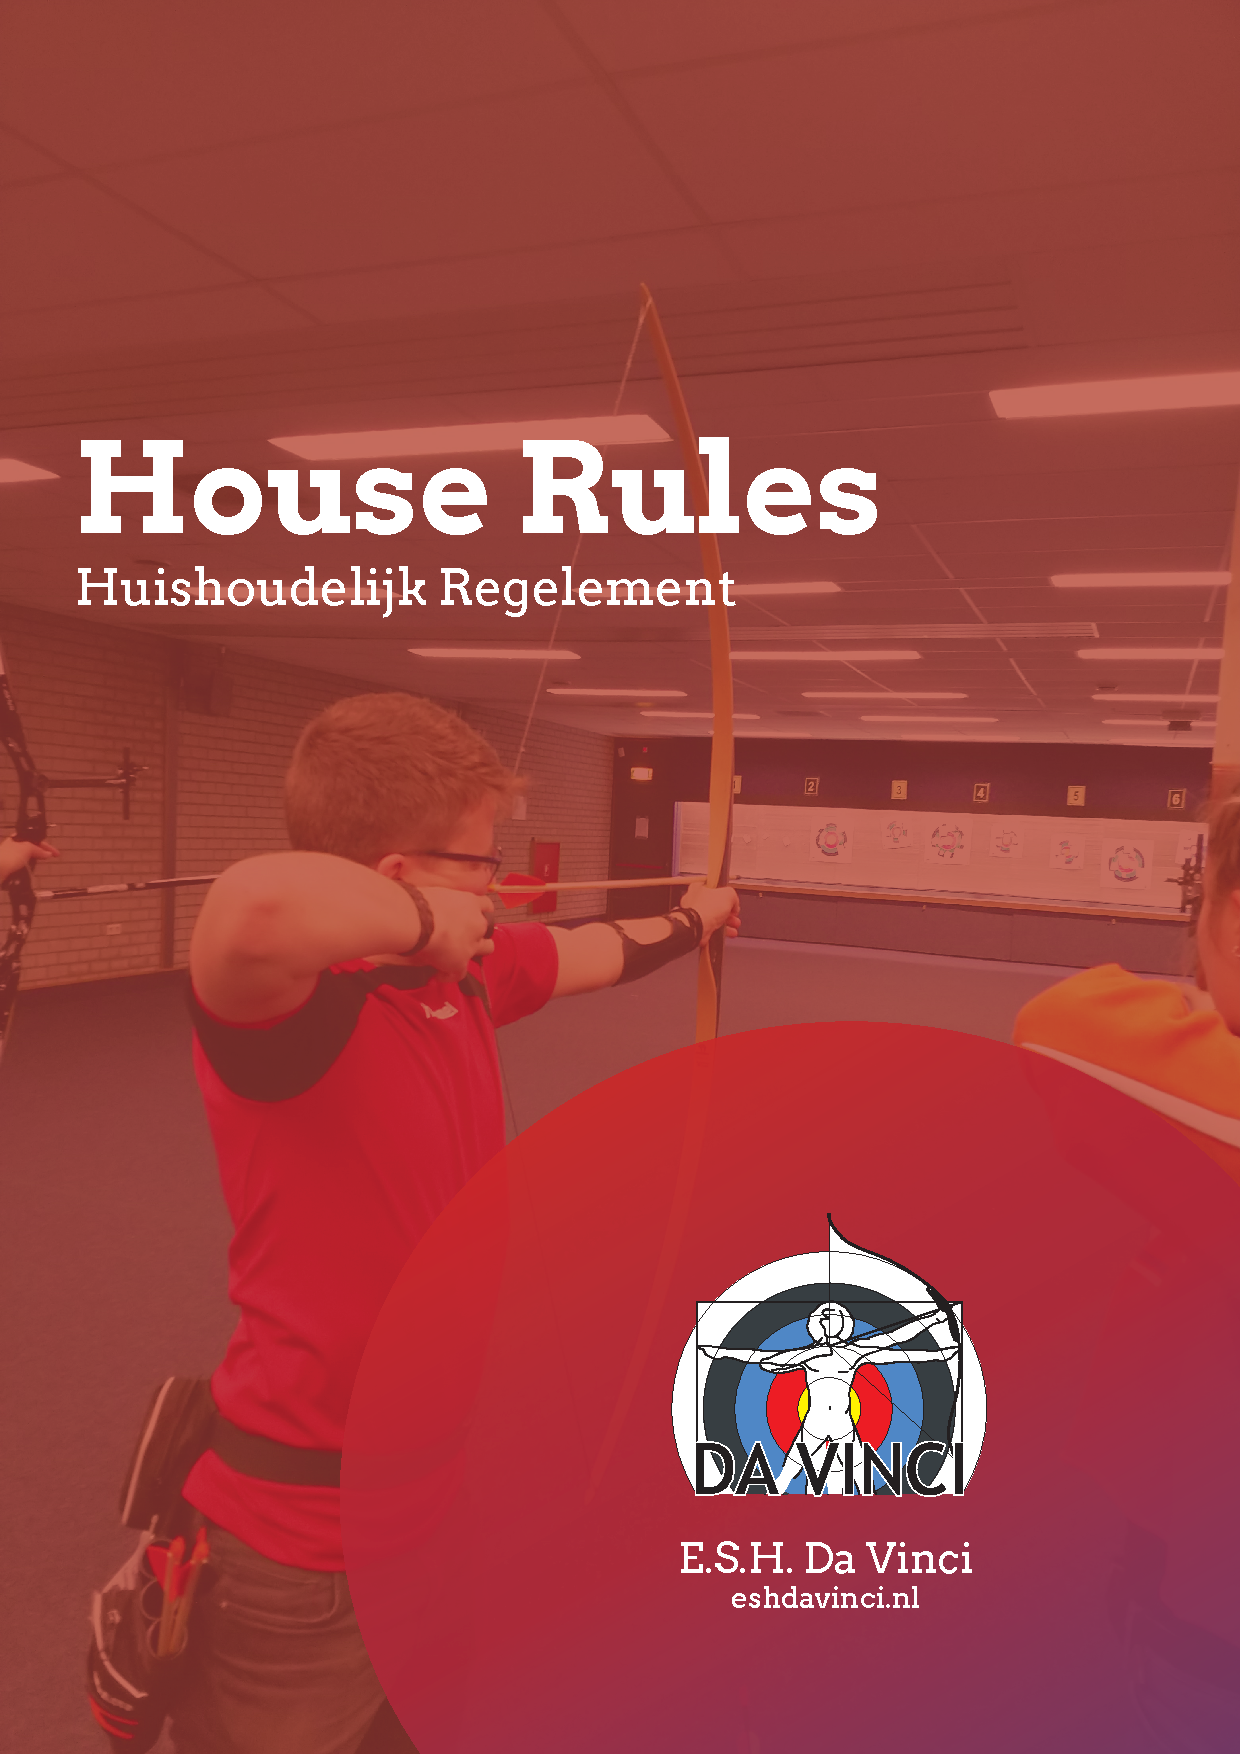
\includepdf[fitpaper=true, pages=-]{Cover.pdf}
\tableofcontents
\pagebreak
\section*{List of Definitions}
{\g Definitions can be recognized by the capital letter at the start throughout this document. Board Member roles are also spelled with a capital (Chairman, Secretary, Treasurer)}

\bigskip

\begin{description}[font=\sffamily\bfseries, leftmargin=1cm, style=nextline]
  \item[GA]
    General Assembly or General Members Meeting (ALV)
  \item[BM]
    Board Meeting (BV)
  \item[Workshop]
    An event organized for an external party, with an aim of presenting the sport to outsiders. If desired it is possible to try out archery under guidance of experienced archers.
    \item[ESSF]
    Eindhovense Studenten Sport Federatie (Eindhoven Student Sport Federation)
    \item[HR]
    \Ahr\ (this document)
    \item[NHB]
    Nederlandse Handboog Bond (Dutch Archery Federation)
    \item[SSC]
    Student Sports Centre Eindhoven (also SSCE)
    \item[TU/e]
    Technische Universiteit Eindhoven (Eindhoven University of Technology)
    \item[ADM]
    Aan de Meet, the association in charge of the maintenance and renting of our Accommodation.
    \item[\Asr]
    The Safety Regulations of E.S.H. Da Vinci can be found in this HR under Chapter 1.
\item[\Abr] Document detailing the actions that the board needs to take during the year.
\item[\Asta] Articles of Association for Da Vinci ("Statuten")
\item[\Awr] Document stating regulations for Contests and Competitions.
\item[\Ajv] Document detailing the actions of the board during the previous year.
    
\item[Member]
Archers that are members of the E.S.H. Da Vinci association. Members are required to have a sport card from the SSC.
\item[External Member]
Archers that are members of the E.S.H. Da Vinci association, but are NHB member through another club.
\item[Recreationist]
Archers that are allowed to take part in trainings. Recreationists are required to have a sport card from the SSC.
\item[Beginner]
Participants to the Beginners' Course
\item[Beginners' Course] Course given to beginners during the year.
\item[Guest] Guests of Da Vinci, this includes Beginners, workshop participants or interested parties.
\item[Honorary Member] Special title given to an archer by the GA for services to Da Vinci.
\item[Experienced - Inexperienced] The Board determines if Archers are experienced, or inexperienced depending on their safety level and skills.
\item[Supervisor] Someone instructing Inexperienced Archers, ensuring safety. Supervisors are: Board Members, official trainers, competition leader(s), and those appointed by the board.
\item[General Training] Training given by the trainers during a defined time.

\item[Accommodation] Our accommodation ("Aan de Meet") consisting of the Shooting Range, Outdoor Range and the Club Room.
\item[Club Room] Also known as “het hok”. It’s the lockable area/room behind the shooting range, assigned for use by E.S.H. Da Vinci.
    \item[Association Year]
    Parallel to the financial year; starting September 1st and ending the 31st of August. 
    
    \item[Shooting Line]
    The line, marked on the floor, from where the archer shoots his arrows towards the target.
    \item[“Behind the line”]
    The side of the Shooting Line where the targets are NOT placed. 
    \item[Waiting Line]
The line placed behind, and parallel to, the Shooting Line. Only supervisors, trainers and participants currently shooting their turn are allowed to be in the space between the Shooting Line and the Waiting Line. 


\item[Downrange of the Line] The area on the side the Shooting Line where the targets are located. Opposite of ``behind the line''.

\end{description}

\pagebreak

\section{Safety Rules}
The shooting range is a safe place, provided that safety rules described here are followed. Every archer must know and observe these rules. We also expect archers to ensure others abide by these rules. \\

Archers violating these rules may be removed from the shooting range. \\

\subsection{General}

\begin{enumerate}
  \item Archers must at all times use common sense and observe the safety of everyone.
  \item All archers must immediately follow safety related instructions from supervisors. The correctness of such instructions is not open for discussion until the instructions have been complied with.
  \item Inexperienced archers are only allowed to shoot under supervision, and should strictly follow all instructions from their supervisors. Experienced archers are allowed to shoot unsupervised.
  \item Aiming a bow at persons or animals is strictly forbidden (even without an arrow on the bow).
  \item When drawing and/or shooting the bow, the angle of the arrow with the ground (elevation) may never exceed 30$^\circ$. Shooting straight up is strictly forbidden.
  \item A drawn bow without an arrow on it may never be released. Doing so may cause the bow to shatter, causing injury and/or damage.
\end{enumerate}

\subsection{Shooting Protocol}

\begin{enumerate}
  \item Bows may only be drawn at the Shooting Line, and only when aimed in the direction of the targets. This also holds when there's no arrow on the bow.
  \item Arrows may only be placed on the bow when at the Shooting Line. The arrow tip must always be pointed in the general direction of the targets, or the ground.
  \item Archers may only take place at the Shooting Line when there is no person Downrange of the Line {\bf and} (for the indoor range) the back door is closed. Until that time, they must wait behind the Waiting Line.
  \item During shooting only active archers and supervisors may be at the Shooting Line. Everyone else, including archers who finished shooting, must wait behind the Waiting Line.
  \item If, during shooting, anyone is found to be Downrange of the Line, or (for the indoor range) the backdoor is found to be open, all archers will immediately stop shooting. Shots are aborted, not finished, and the arrows must be removed from the bows.
  \item When all archers have finished shooting, everyone may fetch their arrows collectively.
\end{enumerate}

\subsection{Ranges}

\begin{enumerate}
  \item There may be no objects (such as targets or scoring boards) on the floor within 3 meters of the target wall.
  \item There will be no running, jumping, pushing, etc. on the range. Reckless behavior is prohibited.
  \item Bows should be put in the designated areas, or in the bow rack.
  \item Spectators are not allowed downrange of the Waiting Line, unless explicitly permitted by supervisors.
\end{enumerate}

\subsection{Outdoor Range}
\label{rules:outdoor}

\begin{enumerate}
  \item Archers are required to wear closed shoes on the outdoor range to protect against obscured arrows stuck in the grass.
  \item Archers who are shooting on the outdoor range must pay extra attention that all archers have returned after fetching their arrows, including those shooting at the 70 or 90 meter targets.
\end{enumerate}

\section{General}
\subsection{Goal and Scope of the \Ahr}
These \Ahr\ supplement the \Asta\ with regards to rules and conditions contributing to the day-to-day functioning of the association. Members (including the board) and Recreationists are tasked with knowing the contents of this document and following the described rules, which will be enforced by the board. \\

\subsection{Behaviour}
Members and Recreationists are always obliged follow the rules of the NHB (and World Archery) regarding the sport and competitions, both during Da Vinci hours as well as at external competitions, where these House Rules do not specify otherwise, as specified in \Asta\ Section 4.4. \\

Archers are expected to behave appropriately and to not embarrass Da Vinci as long as they are in direct association of Da Vinci. This includes that archers who participate in external competitions will show good sportsmanship, follow up the (safety) rules and regulations for that competition. While not mandatory, assistance at and supporting activities organized by the association is highly appreciated. \\

Further regulations about safe behavior on the shooting range, as well as general competition rules, are part of the \Awr\ and the \Asr .

\subsection{Clothing Rules}
\label{section:clubclothing}
At regional and team competitions, organized by the NHB, (non-External) Members are required to wear a club shirt, together with a black pair of pants without any markings. This rule also applies if one is representing Da Vinci, for instance during the intro, the Beginners' Course or at another competition where one is using the Da Vinci name, or present with a larger team from Da Vinci. At NHB competitions, the NHB regulations for clothing should be followed as well (and thus all jeans are not allowed).

\subsection{Fines and Suspensions}
\label{rules:ban}
Whenever an Archer infringes upon one or more articles from the \Asta , \Ahr\ or \Asr\, or in case of infringing upon regulations based on the rules described in these documents, the board can punish the violator with a fine and/or suspension. The severity of this measure will be determined depending on the specific infringement. In case of disagreement between the board and the violator, the matter will be mediated by a GA.

\subsection{Incorporation of the Association}
The association is incorporated at the Kamer van Koophandel under number 17174167. The association is also a member of the ESSF, based at the SSC, and the NHB under number 1364.

\subsection{Changes to the \Ahr}
Proposals to change the \Ahr\ shall be submitted at least 14 days in advance of the next GA by at least three Members, or the board. An overview of these changes will be communicated by written notice by the board at least 7 days in advance of the GA. Proposed changes to the \Ahr\ will only go into effect after they have been approved by the GA. Changes in the \Asr\ can be implemented directly by the board, without GA approval, as they improve safety. Changes to the \Asr\ have to be discussed in the next GA.

\subsection{Validity of the \Ahr}
The \Ahr\ will be declared invalid upon dissolvement of the association, or when the \Asta\ are changed. Upon changing of the \Asta , the \Ahr\ have to be re-approved to make sure that they do not contradict the \Asta . The \Ahr\ should be checked at least once a year for inconsistencies with day-to-day rules, and updated if necessary. New rules decided upon by the GA should also be added to the \Ahr .

\subsection{Availability of the \Ahr}
\label{section:available}
At least one printout of the \Ahr\ and \Asta\ should always be present at the training location. Every Member and Recreationist is entitled to review these regulations, to make sure that nobody can claim unfamiliarity with these rules. The \Ahr\ and \Asta\ should also be available on the E.S.H. Da Vinci website.

\subsection{\App}
As the association processes personal data for Guests, (External) Members, Beginners, Recreationists and Trainers, a document detailing the processing and storage of personal data, the \App\, needs to be available to all affected, in accordance to the \textit{Algemene verordening gegevensbescherming} (AVG), as entered into Dutch law on the 25th of May 2018.

\subsubsection{Availability}
The \App\ should always be made available together with the \Ahr , as specified in Section \ref{section:available}. All affected, including Guests, are permitted to view this document.

\subsubsection{Changes}
The board is permitted to change the \App\ if regulations change in Dutch law, if contracted third parties require different data for daily functions and if the association requires different data for daily function of the association. Changes for other reasons, such as but not limited to gathering more data for statistical purposes, or the addition of new third parties, requires explicit GA approval. \\

If the \App\ is changed, a written notice stating changes, and distributing the new \App\ will be sent by the board to all affected, including but not limited to Members, Recreationists and Trainers. Affected persons have the right to object to this change by written response within two weeks (fourteen (14) days) of the original notice by the board. If no explicit GA approval was given, explicit GA approval will be required upon objection of an affected person.

\subsection{General Assembly}
\subsubsection{Organization}
\label{section:yearlyGA}
The board is obliged to, as stated in \Asta\ Section 14.1, organize a GA at least once every year and they may organize a GA at any time. The board shall provide an agenda and invitation and send these together with the announcement of the date of the GA. Any GA is convened by written notice to all Members and Recreationists within a period of at least seven days as specified in \Asta\ Section 15.3. At the yearly GA, the board is obliged to report the \Ajv\ and to present and explain the Realization, in accordance to the \Asta\ Section 14.1. \\

As stated in \Asta\ Section 15.2, the board can be required to organize a GA within two weeks, if at least one tenth of the Members, eligible for voting at the GA, request them to do so. The normal procedure for GA announcement, as detailed above, will then be followed. If the board fails to organize a GA, the requesters will choose their own chairman for this GA, who will send the written notice to all Members and Recreationists. \\

\subsubsection{Voting}
The voting or poll takes place as a rule by show of hands and in person, or by proxy (you can vote by proxy for only two Members, as specified in \Asta\ Section 12.2). If the board, or at least one Member or Recreationist deems it desirable, the chairman may decide to a written vote or poll, in accordance to \Asta\ Section 12.4. If a vote or poll concerns people (for instance the choosing of a new board), it shall always be a written vote. \\ 

In the event of a written vote, the chairman designates a voting committee consisting of two members. The board provides authenticated voting papers. The numbers of voting papers handed in must be equal to the numbers of voting members present, combined with the amount of votes by proxy. The committee counts the votes and checks the validity of the votes. The committee will announce the result of the vote to the GA. \\

A voting ballot shall be declared invalid in case of the following: it is signed, the paper is not marked by the board, the ballot is unreadable/unclear or if it contains a choice that was not part of the set of choices that is currently being voted on.

\section{Members and Recreationists}
\subsection{Requirements}
All Members and Recreationists are required to conform to the SSC rules for joining sports associations, including, but not limited to, the rule requiring a valid student sport card.

\subsection{Guests}
Guests are people who are not associated with Da Vinci, but are invited to be present at the range. This includes spectators and archers shooting in workshops.

\subsection{Beginners}
Beginners are Archers participating in the Beginners' Course. Beginners are not Members of the club, but they are required to have a valid sports card. Beginners are by definition Inexperienced Archers.

\subsection{Members}
Members of Da Vinci, as defined in \Asta. Members are required to be NHB member and to have a valid sports card. Members have the right to attend GAs and vote there.

\subsection{External Members}
External Members are a type of Members; they have the exact same rights and obligations, except that they have an NHB membership through another club and not through Da Vinci.

\subsection{Recreationists}
Recreationists are SSC members with a valid sports card who through the SSC are allowed to make use of Da Vinci's facilities and materials. Recreationists are allowed to attend the Beginners' Course, as well as trainings and activities, to be selected by the board. \\

Recreationists are not Members. As a courtesy they are invited to attend GAs as guests; they are not allowed to vote there.

\subsection{Honoraries}
A person who has shown extraordinary effort to support or improve Da Vinci can be nominated as an Honorary Member by the board or at least 5 Members that are eligible to vote on GAs.
The Honorary Membership is awarded by the GA if there is at least a two-thirds majority vote. Honorary Membership can only be awarded if accepted by the nominee. \\

The Honorary Membership is for life, unless a GA dissolves the Honorary Membership with a two-thirds majority vote. Honorary Members have the right to attend and speak at GAs, but they do not receive a vote. They are also welcome to join (internal) competitions and club activities. When not registered as either a Recreationist or Member, Honoraries cannot attend regular training. \\

The Honorary Membership is a title unrelated to normal membership. However they can also be regular Members assuming they satisfy the relevant conditions. In this case, they also pay a reduced fee.

\subsection{Contribution}
Members and Recreationists have to pay the yearly contribution, within two weeks of being requested to do so. If a Member or Recreationist fails to do so, the board may (temporarily) ban them from Da Vinci. \\

Where applicable, the contribution includes the NHB fee. Da Vinci will pay the NHB fee on behalf of the member. \\

Members or Recreationists wanting to join after the end of the second TU/e quartile are charged a reduced fee. \\


\bigskip
\begin{tabular}{lllll}
                         & \textbf{Fee} & \textbf{Half Year} & \textbf{Honorary} & \textbf{Half Year + Honorary} \\
\textbf{Recreationist}   & €40,-        & €20,-              & -                 & -                             \\
\textbf{External Member} & €40,-        & €20,-              & -                 & -                             \\
\textbf{Member}          & €75,-        & €55,-              & €35,-             & €20,-                        
\end{tabular}

\bigskip

It is also possible to become a financial donor, as specified in the \Asta\ Section 6. The minimal donation to become a financial donor is €20,-. As specified in \Asta\ Section 6.3, donors have the right to attend the General Assembly, but do not have the right to vote. They are also not allowed to join any activities or training.

\section{Board}
More information about the actions that the board needs to take are detailed in the \Abr .
\subsection{Communication}
\subsubsection{Between boardmembers}
The board has to hold meetings (BM) as often as the chairman or two other board members find this necessary.

\subsubsection{To the association}
The board needs to communicate all information that is important for Members and Recreationists and the association, to all Members, Recreationists and trainers. All general notifications need to be posted on the website. Personal messages need to be emailed to the person in question, such that they can be archived. Official documents and announcements, such as GA Agenda, Minutes, etc, need to be communicated per email. \\
 
All upcoming activities and up to date training times need to be published on the website. 
General announcements, updates about upcoming activities and urgent changes in planning will also be communicated via the main communication method, currently the Da Vinci Info App in the Whatsapp application {\g (2019)}.

\subsection{Opening and Closing}
The board is responsible for opening and closing of the accommodation on club evenings. Exceptions to regular opening times must be communicated via the website and other main methods of communication at least one week before the exception. The board is allowed to close early if:

\begin{enumerate}
\item There are no active archers on the shooting range.
\item They have notified the early closure on a main mode of communication.
\item There are no objections within 30 minutes after notification.
\end{enumerate}

\subsection{Election}
A new board is elected during the yearly GA, as specified in Section \ref{section:yearlyGA}, or during any other GA, if there is no board. At least three weeks before the GA, the board will notify all Members and Recreationists with a prior notification that a GA will be held where a board will be elected. Candidates must apply for a board position by written notice to the secretary of the current board within one week of the prior notification. The board will make the candidates known at the time the agenda for the GA is send. Only Members may be board candidates. \\

If there are enough candidates to fill all required board positions by the end of the regular application period, the board will not accept new applications. \\

\subsubsection{Insufficient Candidates}

If there are not enough candidates to fill all required board positions, the board will notify all Members that the application period is extended to the start of the election vote of the GA. \\

If the candidates are not chosen to be board members by the GA, Members can apply for a board position during the GA. If enough candidates are found and a board is chosen it can be installed at the same GA. If no board is chosen, the current board will remain installed.

\subsubsection{Inability to Elect a Board}

If no new board is elected at the GA, the effective board is entitled to suspend all activities including training, free practice and all other club activities until new candidates are found. The board is obligated to organize a GA with the intent to elect and install a new board as soon as enough candidates have applied. \\

If no new board can be found within three months after the original GA, the board is entitled to organize a GA with the purpose to either elect and install a new board or, if no new board can be found, initiate the termination of the association.

\subsection{\Ajv}
The board is required to deliver a \Ajv\ at the end of their board year. This \Ajv\ needs to be discussed and approved at the yearly GA. In this \Ajv\ the board lists all decisions/changes made in the last year, as well as their accomplishments for the association. It should also include a vision for the future of the association.

\pagebreak

\section{Committees}
\subsection{Establishment}
The board can establish a committee with a clear task description by communicating its establishment at a GA or by using a written notice, which includes the task description and the initial committee members, sent to Members and Recreationists.

\subsection{Dissolution}
\subsubsection{Dissolution by the board}
The committee can be dissolved by the board or GA when they have decided that its task is accomplished or obsolete, or if all tasks have been distributed over other committees (or the board). When a committee by the board or GA is dissolved, the board will sent a written notice of dissolution to all Members and Recreationists.

\subsubsection{Dissolution upon task completion}
The committee can also be dissolved automatically, if this was decided at establishment. These committees will be automatically dissolved after they have accomplished their tasks, and are used for one-time events. When such a committee has completed their tasks, a written notice of dissolution will be sent to all Members and Recreationists by the board.

\subsubsection{Dissolution notice}
Dissolution notices for committees should contain a date when the committee will be dissolved and a final report about their tasks.

\subsection{Structure}
Every committee has a chairman, who is responsible for presenting results to the board and maintaining order and effective task execution within the committee. Every committee will also be appointed a board member as a board contact, who will serve as a first contact point, and will stay up to date with current committee tasks.

\subsection{Reporting}
Committees are tasked with reporting their status to the board before every GA. Committees also have to report their status to the board when asked. Committees can present regarding their committee at the GA, provided they provide their report to the board at least 14 days before the GA, such that the board is aware of the contents of the report.

\subsection{Committee members}
\subsubsection{Joining}
Both Members and Recreationists can join committees after approval of the committee chairman. The board or GA can object to new committee members, provided that they supply both the joining member, as well as the committee itself of a written reasonable objection. The committee chairman is responsible for informing the board when members has requested to join the committee.

\subsubsection{Leaving}
Committee members can leave their committee after they have completed or transferred all their tasks. If tasks cannot be transferred to other committee members, the leaving member will have to complete their task first. The committee chairman is responsible for informing the board when members have requested to leave and can decide if one is allowed to leave the committee. \\ 

The board or GA can also force members to leave committees, provided they supply both the leaving member, as well as the committee itself of a written reasoning.

\subsubsection{Disputes}
In case that disputes arise between the board and committees (and its members), the GA will mediate.

\subsection{Budgets}
Committees have to pass every planned purchase by the Treasurer, who will approve or deny requests. Planned purchases totaling to more than €100,- require a Budget to be submitted to, and approved by the board. Budgets totaling more than €350,- have to be approved by the GA.

\subsection{Workgroups}
Committees may have workgroups, which can have members from outside the committee, to take care of a very specific task. These workgroups have a chairman, who is in the committee, and reports to the committee. Budgetting, reporting, joining and leaving go through the committee. Workgroups can be established to take care of one-time tasks within the supervision of a committee, permitting members from outside the committee to help.

\section{Finances}
\subsection{General}
The board is responsible for keeping track of all income and expenses in the financial administration. They are also required to submit the Budget, Balance and Realization to the GA for approval.

\subsection{Club money box}
The club money box is the responsibility of the Treasurer and he/she must ensure that money is only used to purchase goods for the club.

\subsection{Archival}
The Treasurer is also responsible for making sure that receipts and invoices are kept for all purchases, both cash and digital. The Treasurer is also responsible for keeping track of declarations, and making sure they are signed.

\subsection{Purchase of Goods}
The board can purchase goods for the club. Board Members can spend a maximum of €50,- without consultation of the other Board Members, provided it is in the interests of the association. A board majority is necessary to approve a purchase of more than €50,-. In this case the purchase must be discussed and decided on during a BM. \\

When a Budget post is exceeded by €350,-, new purchases require a new Budget, or approval by the GA. All purchases that have not been announced in the Budget, exceeding €350,- need to be approved through a GA to prevent large unannounced purchases by the board.

\subsection{Financial Committee}
The Financial Committee is appointed by the GA to check the execution of the financial policy by the board. It checks the administration of the Treasurer to ensure correctness, traceability and adherence to the submitted Budget. The Financial Committee consists of two committee members. They will be appointed during the yearly GA. One backup committee member will also be appointed. The Committee is, as specified in \Asta\ Section 14.5, entitled to help by a professional, to be paid by Da Vinci, if this is necessary to verify the finances.

\section{Club Materials}
\subsection{Definition}
Club Materials include bows, arrows, personal protection material, spare parts, (outdoor) targets, target faces, other material owned by the club and are used for archery. \\

Club Materials can be used by any person who is permitted by the board to use the materials. The board can always limit usage of Club Materials if needed. The Club Materials are primarily used during the Beginners' Course and Workshops, other usage is permitted only if this activities are not compromised.

\subsection{Maintenance and Repairs}
\subsubsection{Beginners' Course and Workshops}
During the Beginners' Course and Workshops, Supervisors are responsible for inspecting the material for damage at the beginning and end of each training or workshop. Damaged materials must not be used until repaired if safety is compromised.

\subsubsection{General}
The board is responsible for preventative and corrective maintenance of the Club Materials to ensure the materials are safe to use. The board can delegate maintenance to the Material Committee. 

\subsubsection{Damages}
In case of any damage during usage in General Training, free practice or external use, the archer who used the bow is responsible for contacting the board. In case the damage occurred to misuse, the archer is also responsible for repair costs. In case of normal wear and tear it is highly appreciated that archers who use the material play an active role in repairing it.

\subsection{Internal Use}
\subsubsection{Beginners}
Beginners are required to use Club Materials during the Beginners' Course, unless specified otherwise by the board.

\subsubsection{General}
After the Beginners' Course, Members and Recreationists are allowed to use the Club Materials during training and free practice. In case there are not enough bow and/or arrows available, the bows are distributed on a first come first serve basis.

\subsubsection{Costs}
During the first 6 months, using club bows and arrows is free of charge. After 6 months a small fee needs to be paid per club evening (now: 0,50 euro). The board and trainers from the SSC can always claim a bow for instruction purposes. In case someone paid a fee for that bow that evening, the fee will be restituted.

\subsection{External Use}
Members and Recreationists are allowed to borrow Club Material for use in external competitions. When borrowing a fee is required equal to the fee of two evenings for each period between club evenings. If the bow is not returned before the beginning of the next club evening, a fee for that evening needs is required. A deposit of 50 euros needs to be paid, any damage needs to payed from this deposit. In case damage exceeds the amount of the deposit, the member is still required to pay for the damage. \\

In case Club Material is needed for a Beginners' Course, the material needs to be returned in good working order, at the latest at the start of the lesson. In case the material is not in good order or returned too late, a fine of 10 euro is to be paid. If no valid reason is provided for not returning the material in good order on time, the board can decide that the member is no longer allowed to use Club Materials.

\section{Accommodation}
\subsection{Opening Hours}
\label{section:opening}
The Accomodation is opened at the regular training times, which are published on the website and communicated by the board in advance. Regular training times are {\g (2019)}: \\

\begin{tabular}{lll}
Monday    & 18.00-20.00 & Free Practice  and Beginners’ Courses \\
          & 20.00-22.00 & General Training (with a trainer)     \\
Wednesday & 18.00-20.00 & Free Practice and Beginners' Courses  \\
          & 20.00-22.00 & Free Practice                        
\end{tabular}

\bigskip

If all the shooting lanes on the range are in use during a Beginners’ Course, other Members or Recreationists are not allowed to shoot. The board will communicate the dates of the Beginners’ Course to Members and Recreationists.

\subsubsection{Entrance}
On Wednesday evenings Da Vinci is not allowed to use the front door to enter or exit the Shooting Range, instead you can use the back door. If on any other day the front door can not be used, the Board will clearly communicate this to the Archers. 

\subsection{Maintenance and Cleaning}
Members and Recreationists can be requested to help with maintenance and cleaning of the Accomodation by the board. Maintenance costs will be paid for by the association. If necessary, financial help may be asked for from the SSC.

\subsubsection{Small tasks}
Members and Recreationists are expected to perform small maintenance, such as throwing out the trash, themselves without board involvement.

\subsection{Shooting Range}
\subsubsection{Entrance Requirements}
The Shooting Range can be used by Members and Recreationists. Guests need explicit permission from the board to use the shooting range. 

\subsubsection{Allowed Materials on the Shooting Range}
Only hand bows are allowed on the Shooting Range. Shooting with crossbows, firearms or other weapons is forbidden. When introducing a different kind of bow, approval from the board is required. Only arrows with a smooth point are allowed. Arrows with hunting points and/or protrusions and edges at the tip are not allowed.

\subsection{Outdoor Range}
\label{section:outdoor}
The Outdoor Range offers some flexibility around opening hours. If the gates of the Accommodation are open, or the Member is in possession of a gate key, Members can use the Outdoor Range outside regular opening hours under the following conditions:

\begin{enumerate}
\item The Member uses their own material (bow, arrows).
\item The Member is an experienced archer, who is able to hit at least the 30 meter target without problems.
\item The Member needs to be aware of the safety regulations for the Outside Range, as described in Section \ref{rules:outdoor}, and must comply to these rules. Non compliance will lead to punishment, as specified in Section \ref{rules:ban}.
\end{enumerate}

The gates are not always open: if the gates are closed it’s not possible to use the range. If you would like to train outside often, you can request a gate key from the board, who will review the situation and grant or deny the request, possibly against a fee. \\

Use of the Outdoor Range outside regular opening hours by Recreationists or Guests is only allowed in the presence of a board member or a Member approved by the board. In all other situations it is absolutely forbidden for a Recreationist or Guest to train on the outdoor range, outside regular training hours. 

\subsubsection{Gate Keys}
Members can obtain a Gate Key through the Board in exchange for a fee, as specified by the ADM. After receiving a Gate Key, rules from ADM apply regarding the ownership of the key. If a Member is not required to give back the key after the end of their membership, the rules from Section \ref{section:outdoor} still apply, and they will thus not be allowed to use Da Vinci targets.

\subsubsection{Use of Materials from the Club Room}
When using the Outdoor Range outside of Da Vinci opening hours, archers are never permitted to enter the Accommodation, including but not limited to the Club Room, except with express permission from ADM. You will therefore have to bring your own materials to the Outdoor Range, instead of storing them at the Club Room.

\subsection{Club Room}
\subsubsection{Usage rules}
The Club Room may be used by Members and Recreationists at Da Vinci, as well as by participants of the Beginners' Course, as well as those who have been granted access by the board. 

\subsubsection{Safety}
To prevent holdups at the shooting range, the door Downrange of the Line will be closed whenever nobody is present, or when archers are present for longer than a minute. The door will only be reopened after knocking, in accordance with the \Asr .

\subsubsection{Storing personal belongings}
Members and Recreationists are permitted to store their archery equipment, such as bows and arrows in the Club Room in spots destined for storage, as decided by the board. These materials are stored without any insurance policy, and are stored at own risk. The board will ensure safety of stored materials on a best effort basis. Stored items must be labeled with some indication of the owners identity. The board may also request the removal of items with a one month notice.


\section{Training}
\subsection{Beginners' Course}
\subsubsection{Frequency}
A Beginners' Course is organized at least twice per year, or more often if the board decides the external interest and resources are sufficient to organize more courses. At least one course will start in the beginning of the academic year and one course will start in the beginning of the calendar year.

\subsubsection{Duration}
The Beginners' Course consists of 5 classes, which each take 90 minutes. The classes will take place during the times described in Section \ref{section:opening} and will be given in 5 consecutive weeks, if possible. In general there will be no lessons on days the TU/e or Fontys is closed, or in exam weeks. If necessary, the board can overrule this.

\subsubsection{Fee}
Participants of the Beginners' Course are required to pay a fee, which is determined by the GA to be 10 euros {\g (2019)}. The board can decide that a deposit needs to be paid, now determined to be 10 euros {\g (2019)}, which will be given back to the beginner if the beginner attended all lessons, or if the board decides that non-attendance is justified.

\subsubsection{Rules}
Beginners have to follow all instructions provided by the Supervisors. Beginners need to have a valid sport card, issued by the SSC. This sports card needs to entitle them to enroll in student sport associations.

\subsubsection{Trainers at the Beginners' Course}
The board will appoint beginners trainers of the Beginners' Course, trainers can be Members or Recreationists that have sufficient skills in archery.

\subsection{General Training}
\subsubsection{Definition}
Training provided by trainers appointed by the SSC.

\subsubsection{Frequency}
The General Training is given once a week for two hours. The trainers and board determine the exact day and time of the training, which can be found in Section \ref{section:opening}.

\subsubsection{Rules}
To participate in the General Training, you need to be either a Member or Recreationist, and follow directions from the trainers and the board. If one decides to not join the General Training, one is obliged to not hinder the training. 

\subsection{Free Practice}
During Opening Hours (Section \ref{section:opening}) when there is no training or activity, you are allowed to shoot freely (called: Free Practice). The board may limit the free practice hours in times of expected low participation, or if activities need to be scheduled during that time. \\

To join the Free Practice you need to be either a Member or Recreationist, and follow directions from the board. You'll also need to be able to exercise archery without extensive supervision in a safe way (Experienced Archer). The board and trainers can decide to allow Guests to participate in the free practice.

\section{Competitions and Activities}
\subsection{General}
All internal competitions and activities are considered to be a training. Both Members and Recreationists can participate. Additional regulations for competitions are described in the \Awr .

\subsection{Internal Competitions}
The board (or the Competitions Committee) is at least required to organize the following internal competitions: \\
\begin{enumerate}
\item \textbf{Ladder competition}: During every academic year a ladder competition is held, open to all Members and Recreationists.
\item \textbf{Koningsschieten}: Koningsschieten is held in the week of the founding of Da Vinci, as close as possible to the 2nd of February.
\end{enumerate}

\subsection{External Competitions}
\subsubsection{Yearly NHB competitions}
The NHB organizes two yearly competitions, bondscompetities, one on 18 meters and one on 25 meters. Each competition consist of a number of matches in the region (regiocompetitie), rayon and national. Da Vinci Members can participate in these competitions both individual as in teams. The board is responsible to notify Members that they can participate, the board is also responsible for subscribing Members and teams. In case Members participate in one of these competitions, the board will publish competition dates on the website. During the whole competition members are required to wear the club clothing, as described in Section \ref{section:clubclothing}.

\subsubsection{Other competitions}
The board should relay invitations to other competitions and publish dates. The board may organize that a group of members participates in such a competition.
\end{document}